\chapter{Quantum Teleportation}

In quantum teleportation, the properties of quantum entanglement are used to send a qubit between observers without physically moving the involved qubit. The qubits themselves are not really teleported, but the state of one qubit is destroyed on one side and extracted on the other side, so the information that the state encodes is communicated. The usefulness of quantum teleportation lies in its ability to send quantum information arbitrarily far distances without exposing quantum states to thermal decoherence from the environment or other adverse effects.

\section{Results} \label{sec:teleResults}
The following qubit state  $|\Psi \rangle = \alpha |0 \rangle + \beta |1 \rangle$ needs to be transferred. By taking advantage of two classical bits and an entangled qubit pair, the state $|\Psi \rangle$ can be transferred.

The following steps were followed to create an entanglement protocol and to perform quantum teleportation.

\textbf{Step 1:} Use a third party entangled qubit pair.

Qubit q$_1$ and qubit q$_2$ were entangled by applying CNOT gate after applying a Hadamard gate, shown in Figure \ref{step1}. These two qubits were used as the ``third party entangled qubit pair''.
\begin{figure}[H]
\centering
\begin{tabular}{c}
\begin{minipage}[c]{.45\linewidth}
\begin{minted}[fontsize=\small
frame=lines,framesep=2mm,baselinestretch=1.2,bgcolor=LightGray,fontsize=\footnotesize,linenos]{python}
q = QuantumCircuit(4,2)

q.h(1)
q.cx(1,2)

q.draw(output='mpl')
\end{minted}
\end{minipage}
\begin{minipage}[c]{.1\linewidth}
\centering
$\rightarrow$
\end{minipage}
\begin{minipage}[c]{.4\linewidth}
\centering
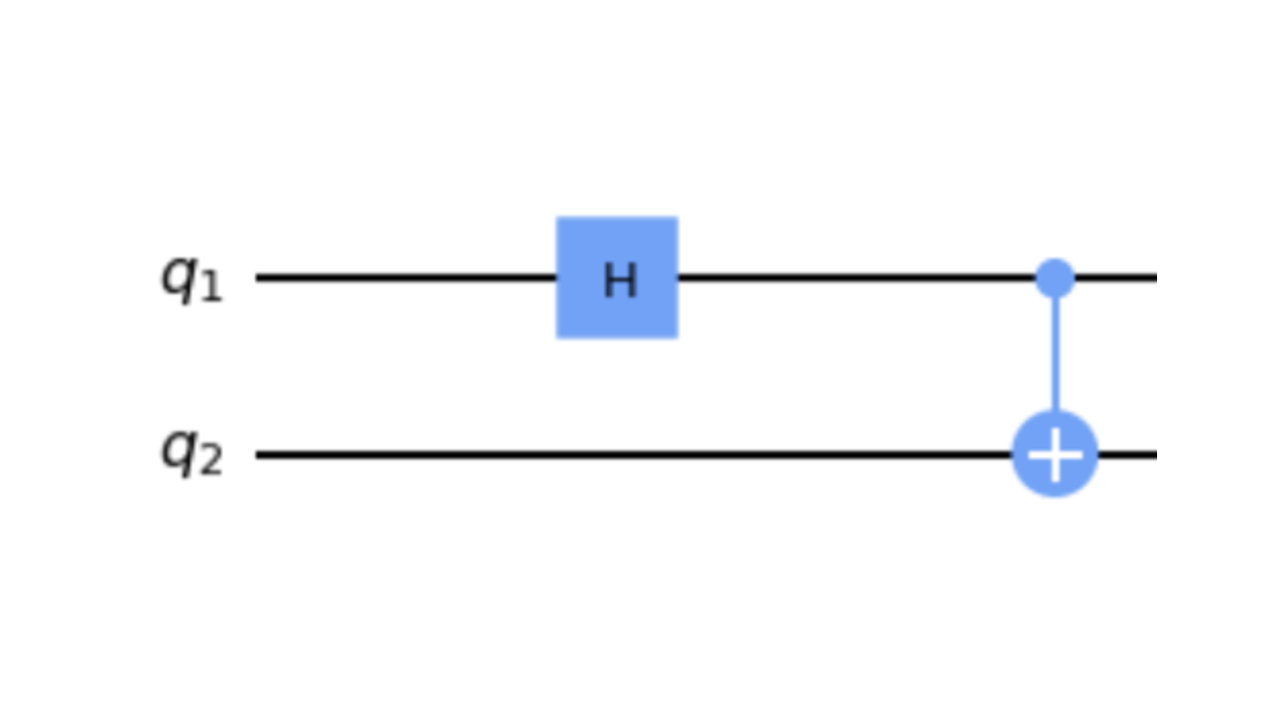
\includegraphics[width=\textwidth]{lab3/images/Step1.png}
\end{minipage}\\
\\ 
\end{tabular}
\captionsetup{font = it, labelfont = bf, width=.91\linewidth, justification=centering}
\caption{Code and circuit diagram to produce entangled pair}
\label{step1}
\end{figure}

\textbf{Step 2:} Perform operations on the qubit that must be sent.

q$_0$ is the qubit that is required to be sent. It is initalised in a random state and then entangled with qubit q$_1$ (one of the third party entangled pairs), shown in Figure \ref{step2}. 

\begin{figure}[H]
\centering
\begin{tabular}{c}
\begin{minipage}[c]{.45\linewidth}
\begin{minted}[fontsize=\small
frame=lines,framesep=2mm,baselinestretch=1.2,bgcolor=LightGray,fontsize=\footnotesize,linenos]{python}
q = QuantumCircuit(4,2)

psi = random_statevector(2)
q.append(Initialize(psi), [0])

q.cx(0,1)
q.h(0)

q.draw(output='mpl')
\end{minted}
\end{minipage}
\begin{minipage}[c]{.1\linewidth}
\centering
$\rightarrow$
\end{minipage}
\begin{minipage}[c]{.4\linewidth}
\centering
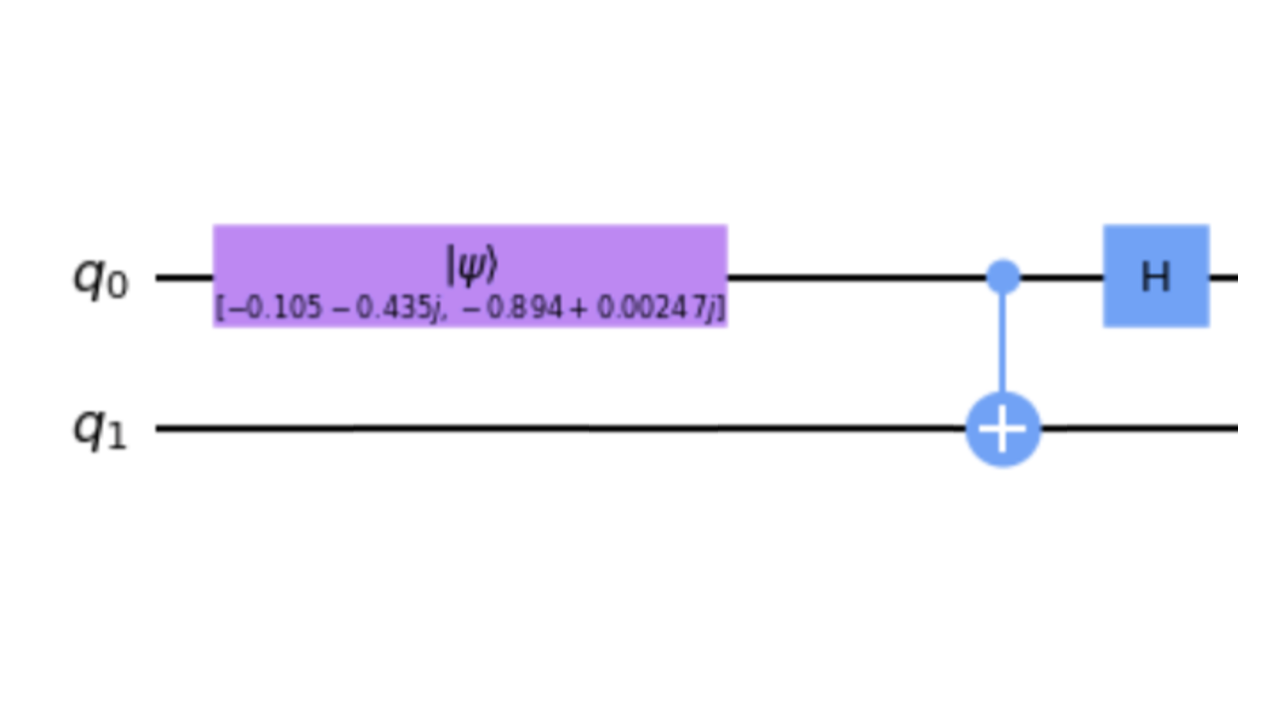
\includegraphics[width=\textwidth]{lab3/images/Step2.png}
\end{minipage}\\
\\ 
\end{tabular}
\captionsetup{font = it, labelfont = bf, width=.91\linewidth, justification=centering}
\caption{Code and circuit diagram to entangle qubit to one of the third party entangled qubits}
\label{step2}
\end{figure}


\textbf{Step 3:} Send the results over a classical communication channel.

The qubit being sent, q$_0$, and one of the third party entangled pair qubits, q$_1$, were measured, stored in classical bits, and sent over a classical communication channel, as can be seen in Figure \ref{step3}.

\begin{figure}[H]
\centering
\begin{tabular}{c}
\begin{minipage}[c]{.45\linewidth}
\begin{minted}[fontsize=\small
frame=lines,framesep=2mm,baselinestretch=1.2,bgcolor=LightGray,fontsize=\footnotesize,linenos]{python}
q = QuantumCircuit(4,2)

q.measure(0,0)
q.measure(1,1)

q.draw(output='mpl')
\end{minted}
\end{minipage}
\begin{minipage}[c]{.1\linewidth}
\centering
$\rightarrow$
\end{minipage}
\begin{minipage}[c]{.4\linewidth}
\centering
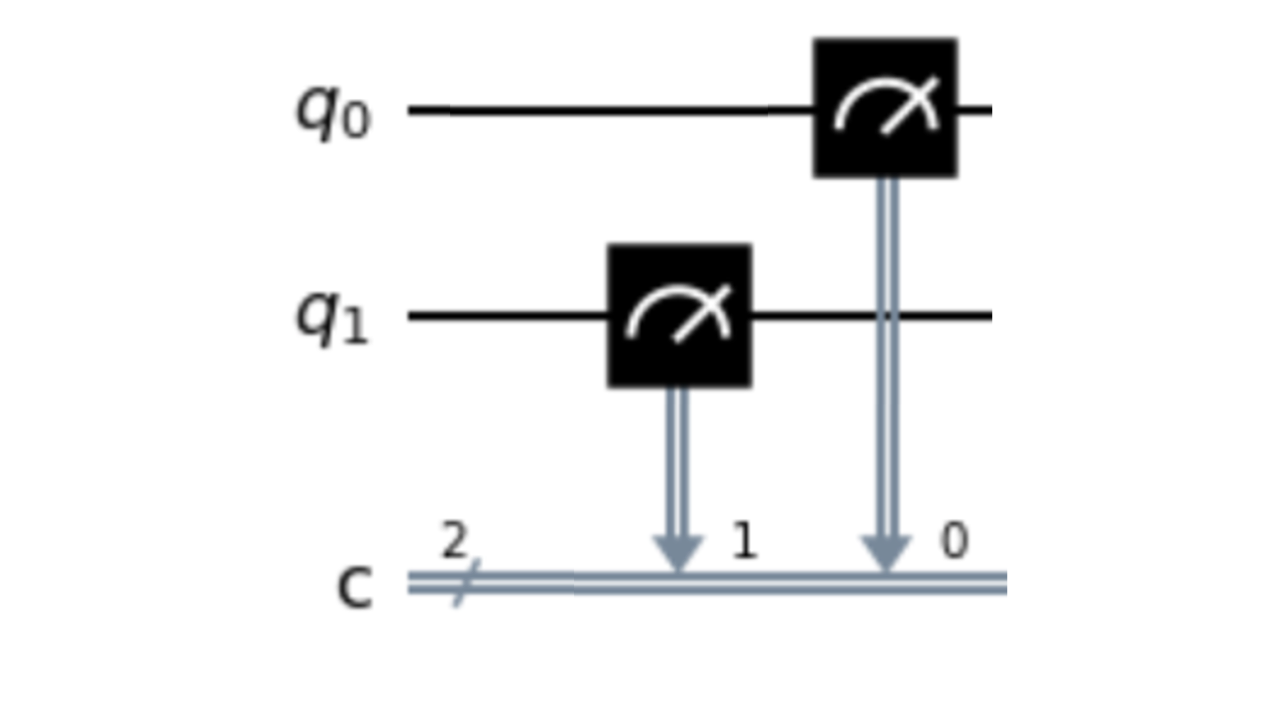
\includegraphics[width=\textwidth]{lab3/images/Step3.png}
\end{minipage}\\
\\ 
\end{tabular}
\captionsetup{font = it, labelfont = bf, width=.91\linewidth, justification=centering}
\caption{Code and circuit diagram to send data over classical channel}
\label{step3}
\end{figure}

\textbf{Step 4:} Perform some operations on the received information to receive the qubit.

The classical bits were received and were used to determine what gates had to be applied to the other third party entangled qubit, q$_2$. 
\begin{itemize}
    \item If 00 is received, then no gates are applied to qubit q$_2$
    \item If 01 is received then an X gate is applied to qubit q$_2$
    \item If 10 is received then a Z gate is applied to qubit q$_2$
    \item If 11 is received then an X gate and a Z gate is applied to qubit q$_2$ in series
\end{itemize}
The implementation can be seen in Figure \ref{step4}.

\begin{figure}[H]
\centering
\begin{tabular}{c}
\begin{minipage}[c]{.45\linewidth}
\begin{minted}[fontsize=\small
frame=lines,framesep=2mm,baselinestretch=1.2,bgcolor=LightGray,fontsize=\footnotesize,linenos]{python}
q = QuantumCircuit(4,2)

q.x(2).c_if(1, 1)
q.z(2).c_if(0, 1)

q.draw(output='mpl')
\end{minted}
\end{minipage}
\begin{minipage}[c]{.1\linewidth}
\centering
$\rightarrow$
\end{minipage}
\begin{minipage}[c]{.4\linewidth}
\centering
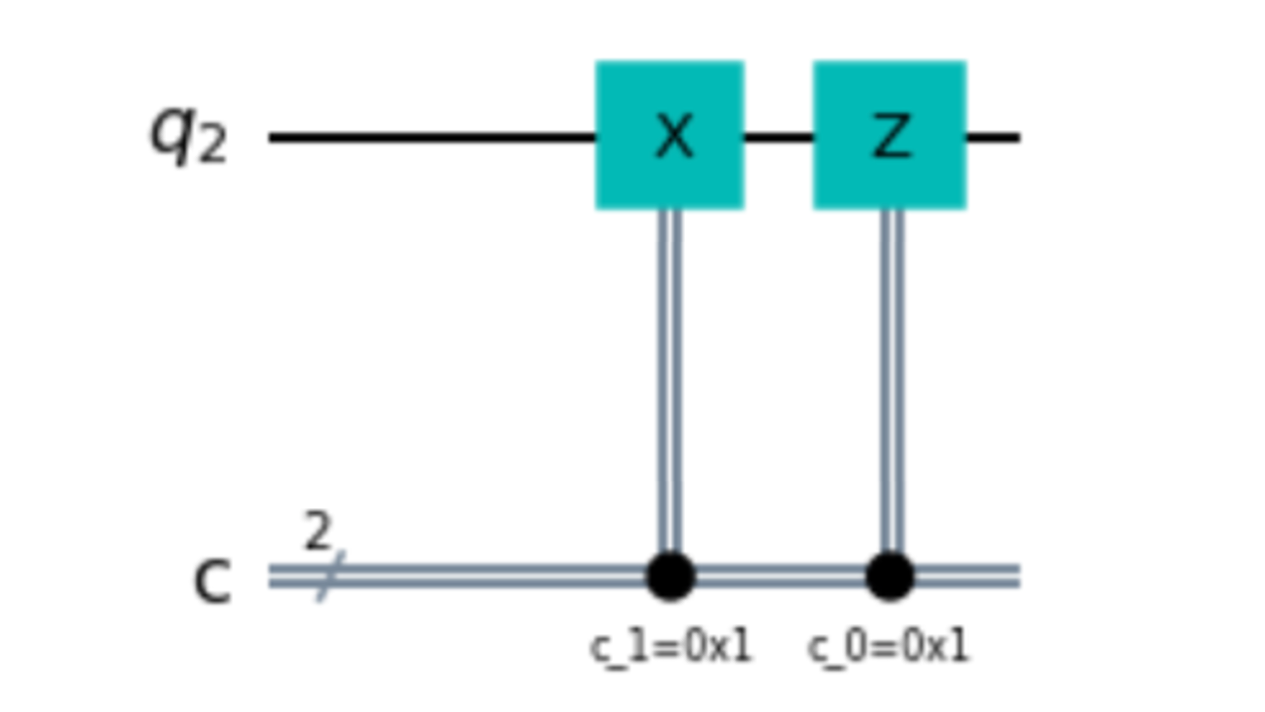
\includegraphics[width=\textwidth]{lab3/images/Step4.png}
\end{minipage}\\
\\ 
\end{tabular}
\captionsetup{font = it, labelfont = bf, width=.91\linewidth, justification=centering}
\caption{Code and circuit diagram to reproduce qubit q$_0$}
\label{step4}
\end{figure}

\subsubsection{Final Design}
The circuit written to perform `quantum teleportation' is shown in Figure \ref{fig:teleportCircuit}.
\begin{figure}[H]
    \centering
    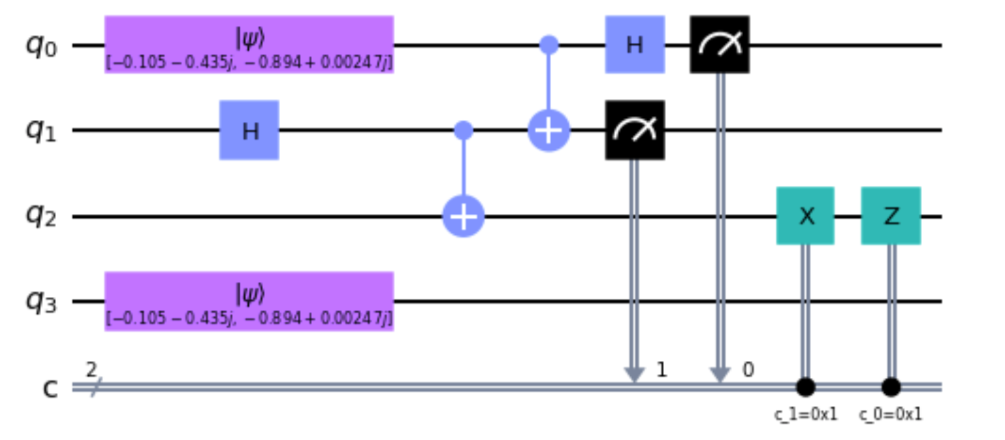
\includegraphics[width=0.6\textwidth]{lab3/images/teleportCircuit.png}
    \captionsetup{font = it, labelfont = bf, width=.91\linewidth, justification=centering}
    \caption{Circuit diagram to teleport qubit q$_0$ to qubit q$_2$, made using qiskit}
    \label{fig:teleportCircuit}
\end{figure}

Qubit q$_3$ was initialised to be the same as qubit q$_0$ (the qubit that was being quantum-mechanically teleported). This was done purely to ensure the same qubit was extracted. Qubit q$_2$ is the qubit that was extracted after teleportation. It is clear that qubit q$_2$ is the same as qubit q$_3$, thus proving the circuit worked. To verify the robustness of this design, the circuit was built using IBMs remote quantum computer. The result from which are discussed in Section \ref{sec:discussTeleport}.

\begin{figure}[h]
    \centering
    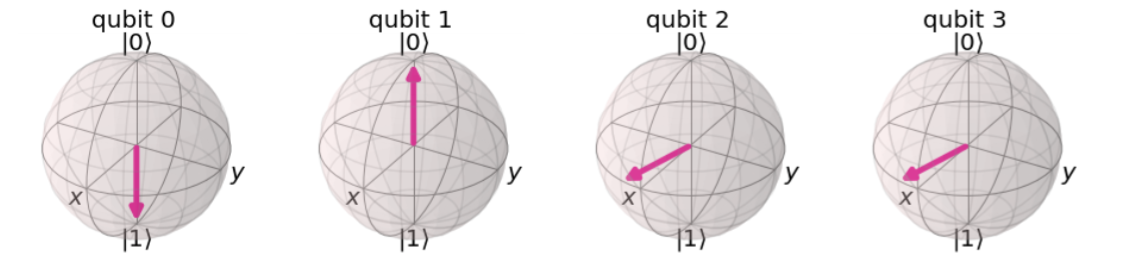
\includegraphics[width=\textwidth]{lab3/images/teleportBloch.png}
    \captionsetup{font = it, labelfont = bf, width=.91\linewidth, justification=centering}
    \caption{Bloch sphere showing the state of each qubit after teleportation has occurred}
    \label{fig:teleportBloch}
\end{figure}

\section{Comparison of Results with Theory}

\begin{figure}[H]
    \centering
    \begin{subfigure}[h]{0.49\textwidth}
        \centering
        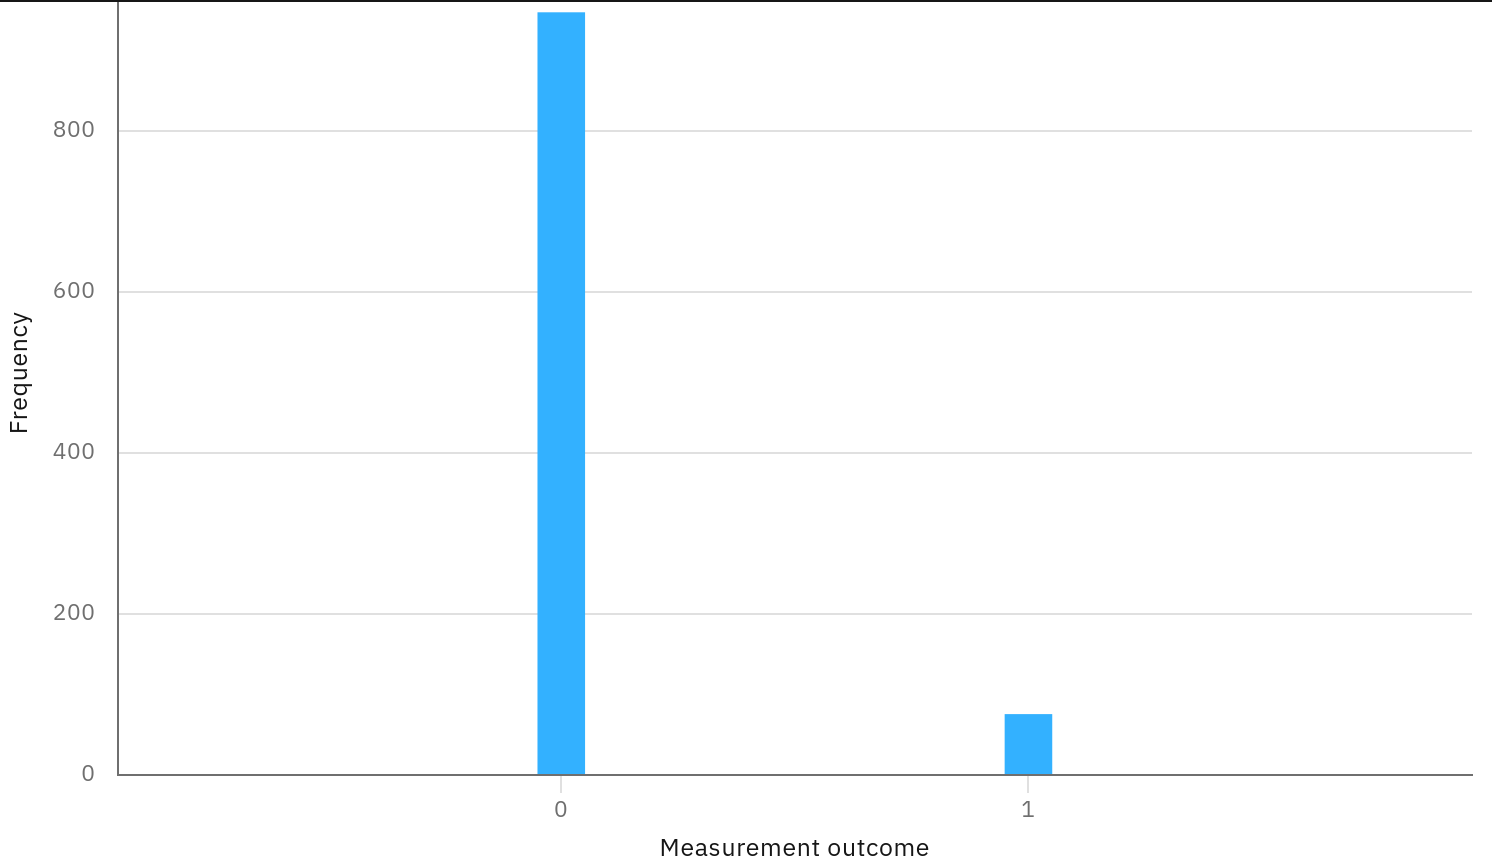
\includegraphics[width=\textwidth]{lab3/images/ibmTeleport.png}
        \caption{}
        \label{fig:ibmHistogramTele}
    \end{subfigure}
    \hfill
    \begin{subfigure}[h]{0.49\textwidth}
        \centering
        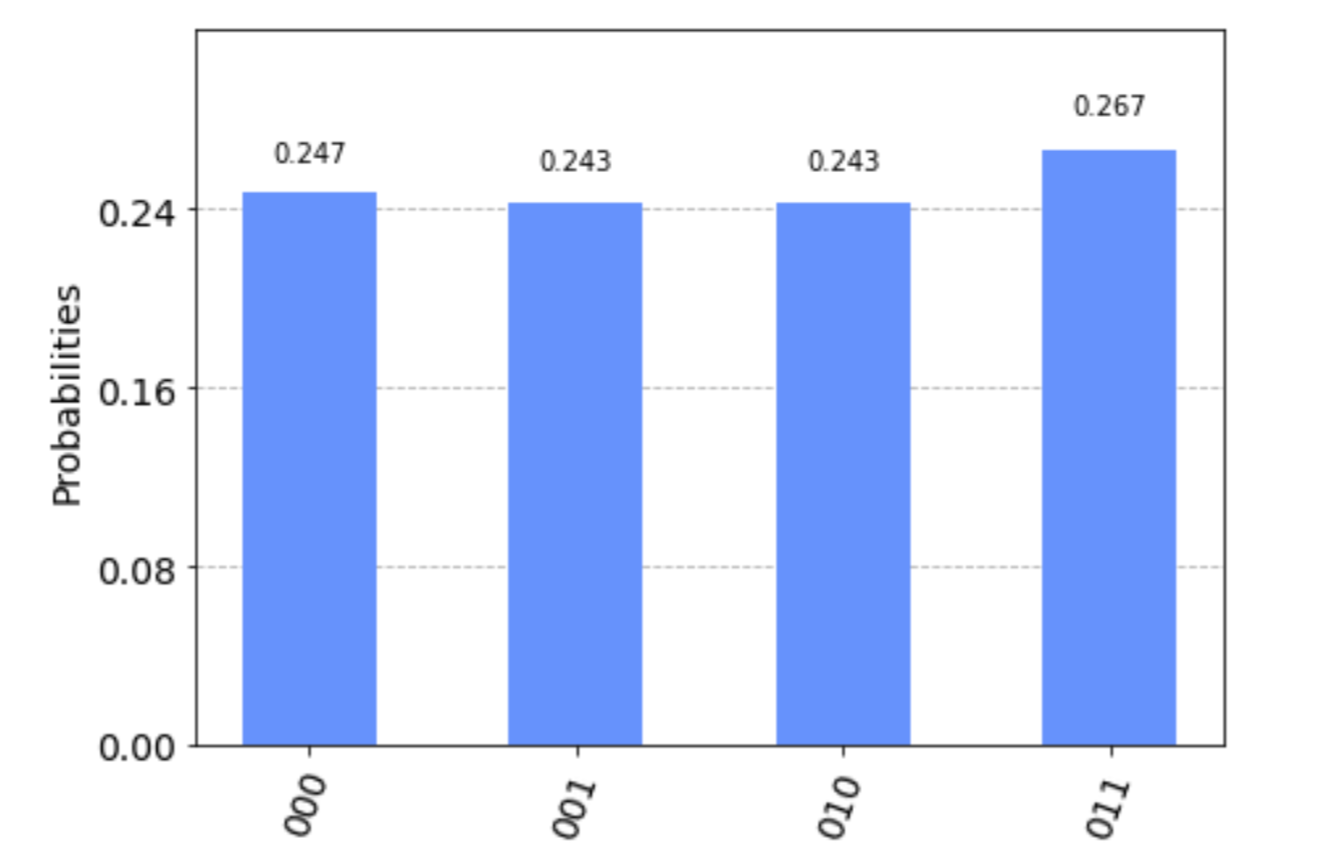
\includegraphics[width=\textwidth]{lab3/images/qiskitHist.png}
        \caption{}
        \label{fig:qiskitHistogramTele}
    \end{subfigure}
    \captionsetup{font = it, labelfont = bf, width=.91\linewidth, justification=centering}
    \caption{Histogram showing a) the probability of measuring each possible state according to qiskit and b) the frequency of the states measured after implementing the circuit using IBM's quantum computer} 
    \label{fig:teleHist}
\end{figure}

A circuit similar to the circuit shown in Figure \ref{fig:teleportCircuit} was implemented in the IBM Quantum Composer environment. The qubit that was required to be teleported was initialized in state $|0\rangle$, instead of a random state, and the results are plotted in Figure \ref{fig:ibmHistogram}. An exact copy of this circuit was implemented using qiskit for comparative purposes, this histogram for which is shown in Figure \ref{fig:qiskitHistogramTele}.

The expected output was for the qubit to always be measured in state $|0\rangle$. This occurred when the circuit was implemented using qiskit (q$_0$ was teleported to q$_2$ which was always measured to be in state $|0\rangle$); however, the qubit was occasionally measured in state $|1\rangle$ when using IBM's quantum computer. The reason for this is discussed in Section \ref{sec:discussTeleport}

\section{Discussion} \label{sec:discussTeleport}
\textbf{Question 1:}
\textit{Follow the steps above, and the knowledge of qiskit you now have from Lab 2 to create a teleportation protocol. You may also benefit from the little revision above which introduce a couple of new features of qiskit}

Steps for teleportation protocol were followed and are discussed in Section \ref{sec:teleResults}. See Figure \ref{fig:teleportCircuit} for the final circuit diagram.

\textbf{Question 2:}

\textbf{2(a)}: \textit{Use IBM composer and compare its results to what you obtained above. Are they different? How so?}


The histogram in Figure \ref{fig:qiskitHistogramTele} shows the result from qiskit. Quantum teleportation was achieved since the qubit being sent, in state $|0\rangle$, was successfully transferred to another qubit when using qiskit. However, this was not the case when implementing the circuit using IBMs circuit. From Figure \ref{fig:ibmHistogramTele}, it is clear that most of the time, the qubit was measured in state $|0\rangle$, but occasionally, the qubit was found to be in state $|1\rangle$. This is due to noise and decoherence affecting the qubit. Qubits are very prone to interference and this can change the state they are in. At some point, between initialisation and measurement, the qubit was corrupted.

\textbf{2(b):} \textit{Now that you have implemented it, what could quantum teleportation be used for and why is it important?}

Quantum hardware is far less robust to errors as classical hardware, since the slightest interaction with the environment causes a qubit to collapse into a discrete state of either 0 or 1. This phenomenon poses significant challenges to the dependability of quantum computers. Using quantum teleportation is extremely important for transferring quantum information to protect it from noise, especially when the information needs to be sent over large distances.
Present-day state-of-the-art quantum computers typically suffer due to decoherence and noise in qubits, hence developing methods to improve the robustness of quantum systems, such as quantum teleportation, is essential for many practical applications.

\section{Conclusions}

In this lab a quantum algorithm was implemented and applied to successfully achieve quantum teleportation. This was first performed using qiskit, and the result was verified by retesting the circuit on IBMs quantum computer. Thus, the objectives were successfully fulfilled. The objectives were achieved with ease, so no changes are necessary to meet those objectives.

To improve understanding, it would be helpful to briefly discuss the quantum algorithm and how it is formed, i.e. the reasons for applying the gates in the given order. Although, having said that, it is understandable if that is outwith the scope of this course.